\section{Results}
Show some results of `simulated' and `realistic' applications.

\begin{itemize}
    \item Fixed road-network, vary MCTS $d$ value
    \begin{itemize}
        \item show SQ get better as $d$ is changed 
        \item show effects of $e$
    \end{itemize}
    \item modify to `random' network, with multiple different variables
\end{itemize}

\subsection{Varying $d$ on the road-network}

\begin{figure}[tbp]
    \centering
    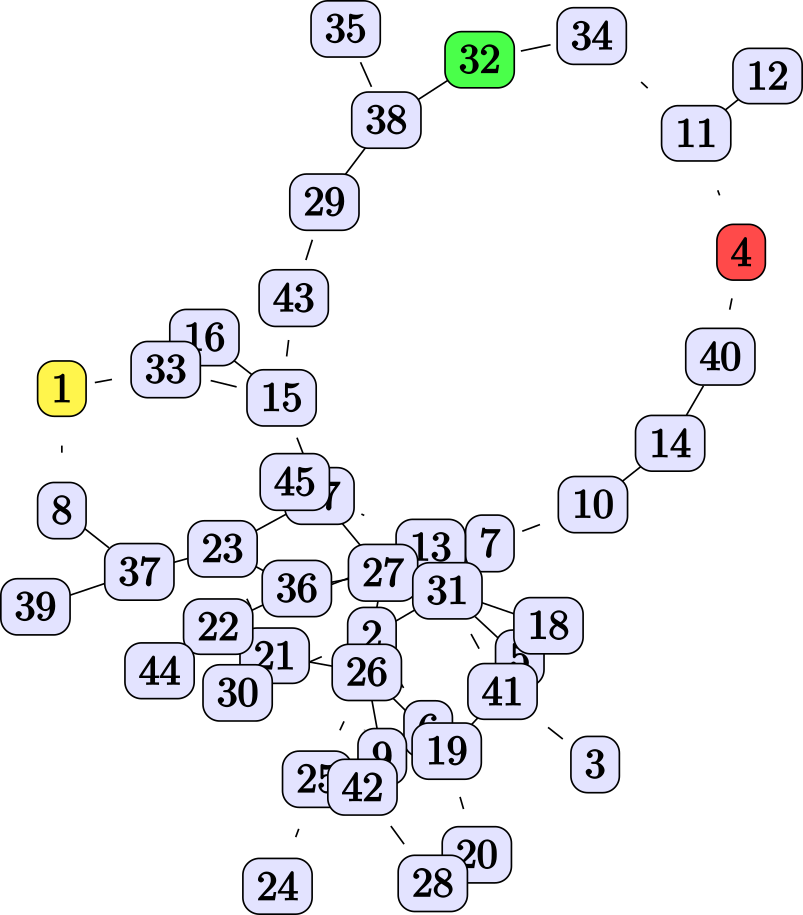
\includegraphics[width=0.4\linewidth]{Figures/medium_roadnet.png}
    \caption{Diagram of a randomly generated road network that is quite a bit larger than the original shown in Figure \ref{fig:roadnet}.}
    \label{fig:med_roadnet}
\end{figure}

In this case we choose the trusted solver to be a MCTS solver with $N=1000$, $D=8$, and $e=1000.0$. For the road network, the transition probability is $p=0.8$ (which means the UGV will travel to the intended location $80\%$ of the time, and a different direction the other $20\%$ of the time). The reward distributions are obtained by running 250 simulations using the same initial conditions.

\begin{figure*}[tbp]
    \centering
    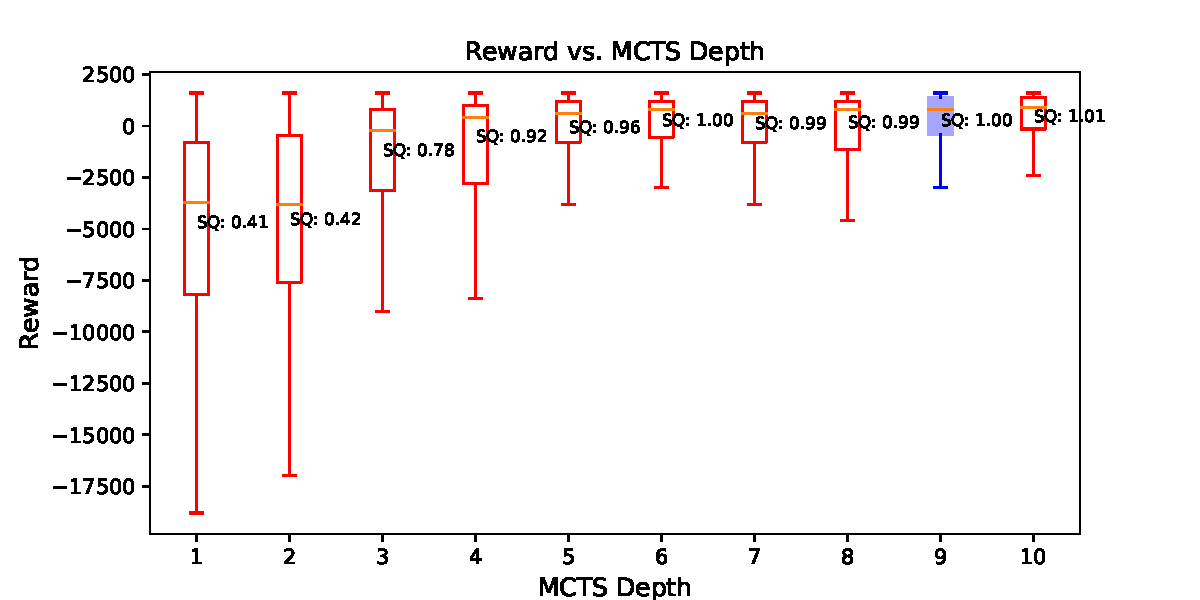
\includegraphics[width=0.6\linewidth]{Figures/sq_roadnet_mcts_i100e1000.pdf}
    \caption{Varying the MCTS `D' parameter for the road network in Figure \ref{fig:roadnet}. Here the solver is using $N=100$ iterations, and an exploration constant of $e=1000$. The SQ values being calculated are with respect to the trusted distribution highlighted, which in this case is the solver with depth equal 9.}
    \label{fig:mcts_d}
\end{figure*}
\begin{figure*}[tbp]
    \centering
    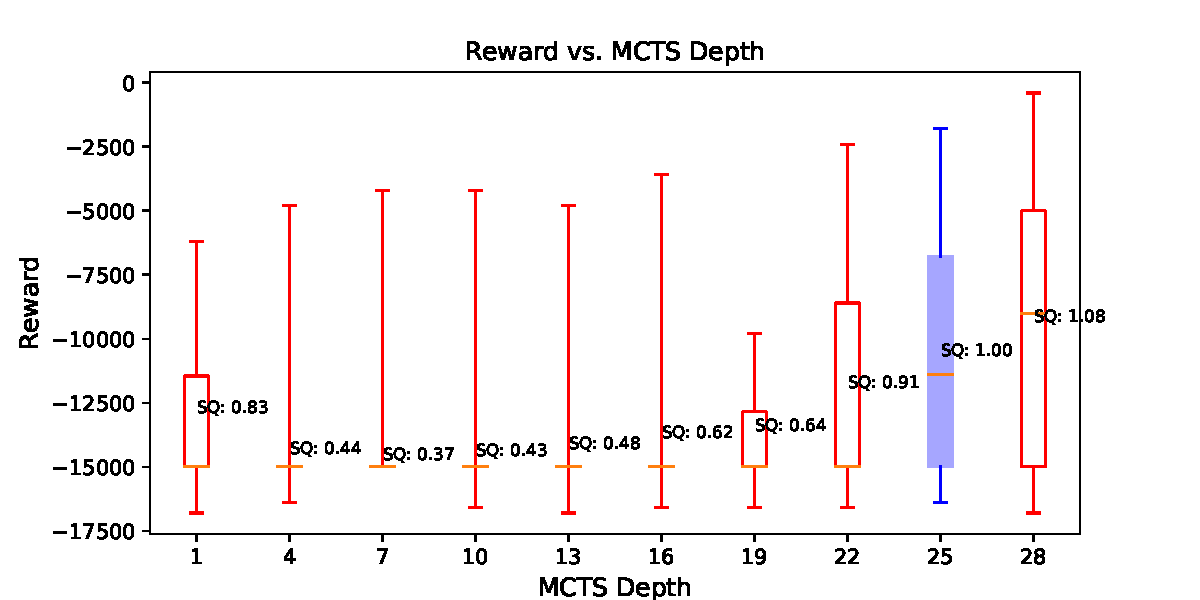
\includegraphics[width=0.6\linewidth]{Figures/sq_mednet_mcts_i1000e2000.pdf}
    \caption{Varying the MCTS `D' parameter for the road network in Figure \ref{fig:med_roadnet}. Here the solver is configured using $N=1000$ iterations and an exploration constant of $e=2000$.}
    \label{fig:mcts_d_med}
\end{figure*}

\begin{table*}
    \footnotesize
    \centering
    \begin{tabular}{lrrrrrrrrr} \toprule
        &\multicolumn{9}{c}{Parameters} \\ \cmidrule(r){2-10}
        Experiment Variables & Network &p_{transe}&e_{mcts}&d_{mcts}&N&rwd_{exit}&rwd_{caught}&rwd_{sense}&its_{mcts} \\ \midrule
        \{p_{trans}\}             & Original & $[0.0,1.0]$ & $[1000.0]$ & 8,3,1 & $[13]$ & 2000 & -2000 & -100 & 1000 \\
        \{p_{trans},e_{mcts}\}      &  Original & $[0.0,1.0]$ & $[10.0,1000.0]$ & 8,3,1 & $[13]$ & 2000 & -2000 & -100 & 1000 \\
        \{N\}                 &  Random & $[0.8]$ & $[1000.0]$ & 8,3,1 & $[8,120]$ & 2000 & -2000 & -100 & 1000 \\
        \{N,p_{trans}\}           &  Random & $[0.0,1.0]$ & $[1000.0]$ & 8,3,1 & $[8,120]$ & 2000 & -2000 & -100 & 1000 \\
        \{N,p_{trans},rwd_{sense}\} &  Random & $[0.0,1.0]$ & $[1000.0]$ & 8,3,1 & $[8,120]$ & 2000 & -2000 & -100 & 1000 \\
        \{rwd_{sense}\}         &  Original & $[0.8]$ & $[1000.0]$ & 8,3,1 & $[13]$ & 2000 & -2000 & $[-5.0,-250.0]$ & 1000 \\
    \end{tabular}
    \caption{Table showing the different parameters used during experiments.}
\end{table*}

\subsection{Varying the transition probability}
In this case a solver quality model was trained using a `trusted' MCTS solver with:

\begin{figure}[tbp]
    \centering
    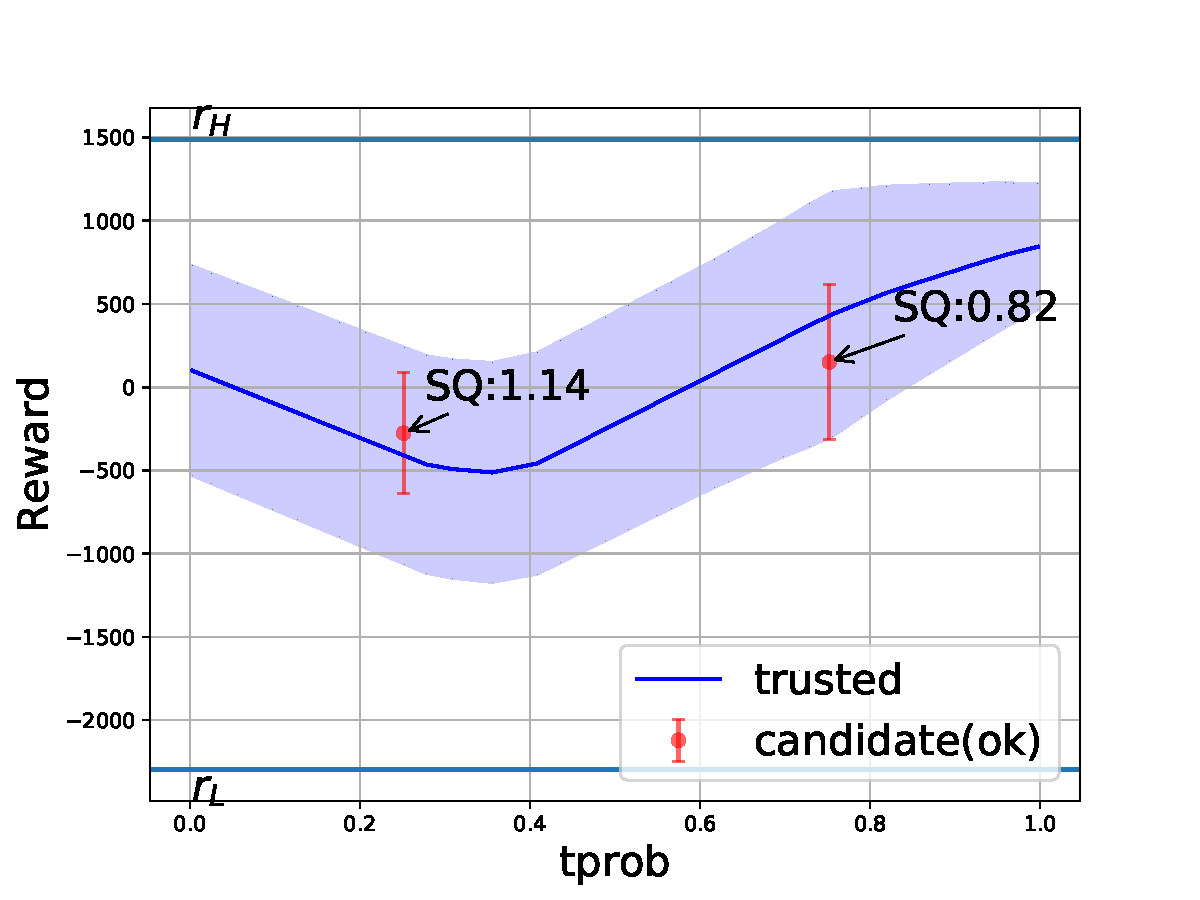
\includegraphics[width=0.9\linewidth]{Figures/transition_vary_tprob_ok.pdf}
    \caption{Using a solver with depth 3}
    \label{fig:tprob}
\end{figure}
\begin{figure}[tbp]
    \centering
    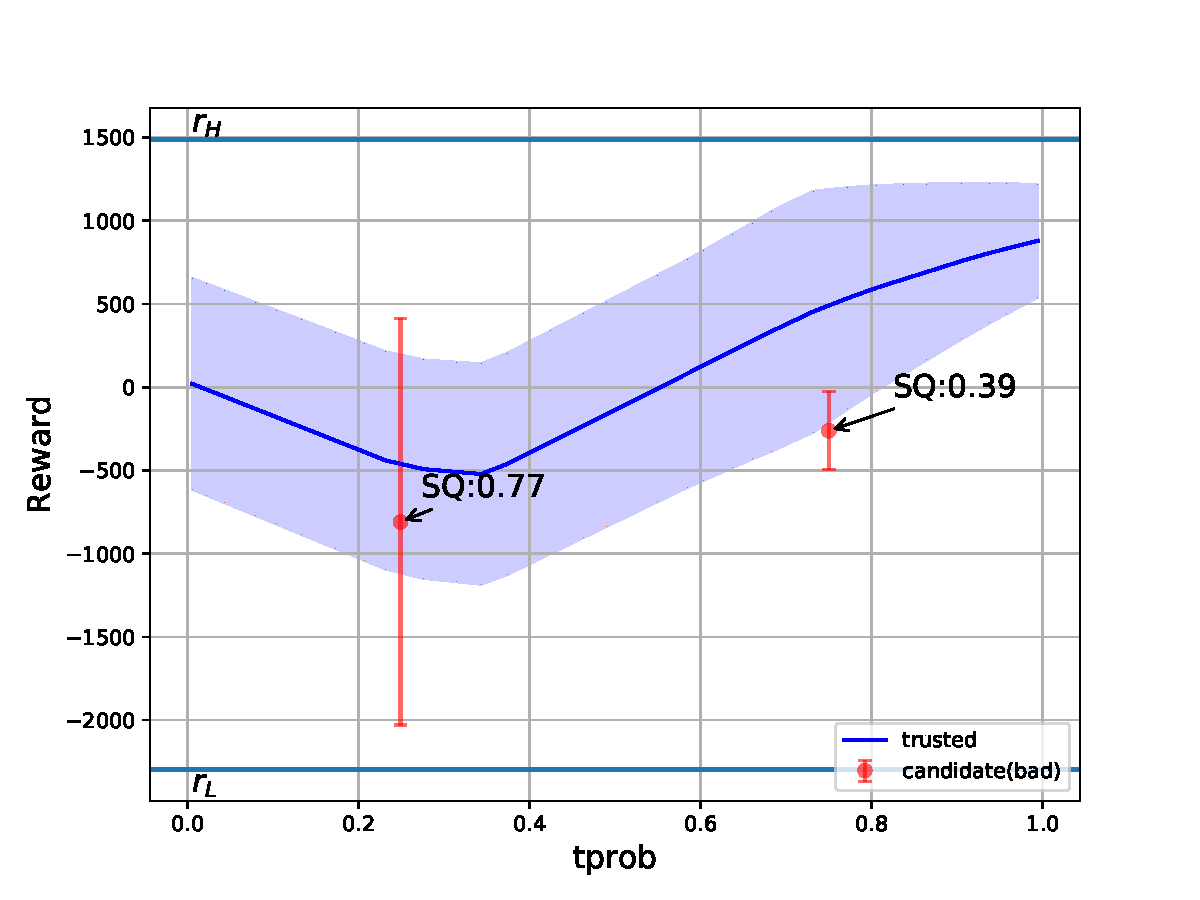
\includegraphics[width=0.9\linewidth]{Figures/transition_vary_tprob_bad.pdf}
    \caption{Using a solver with depth 1}
    \label{fig:tprob}
\end{figure}

\subsection{Varying the transition probability and exploration constant}

\begin{figure}[tbp]
    \centering
    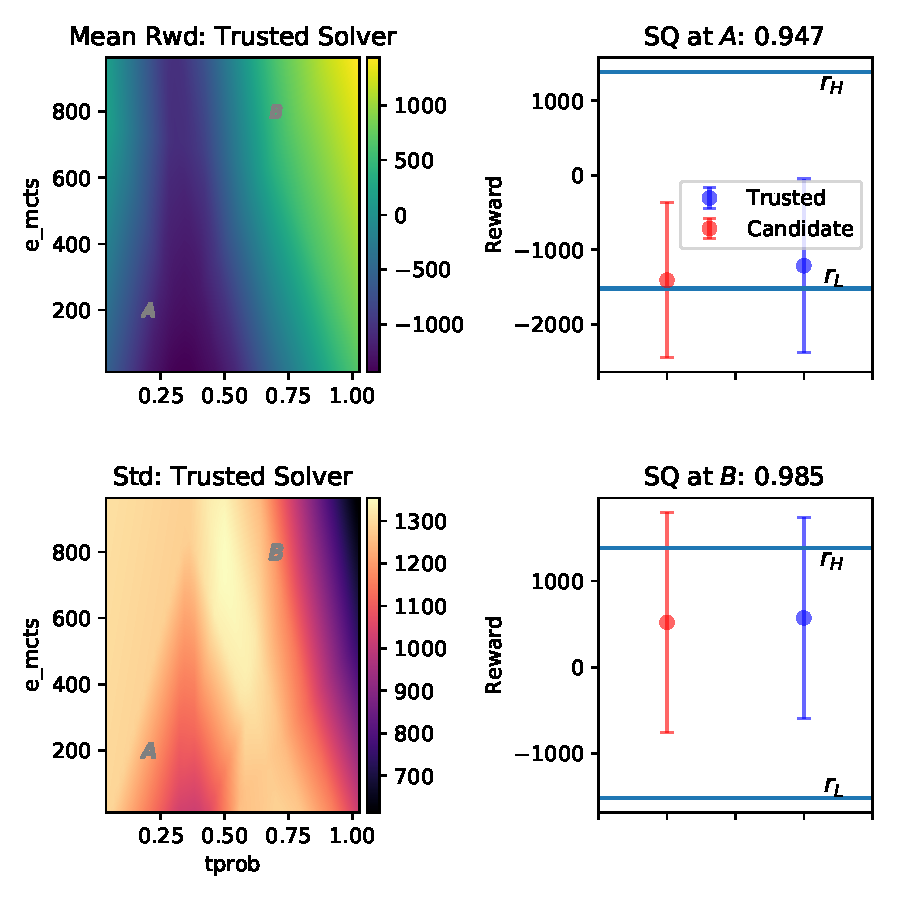
\includegraphics[width=0.9\linewidth]{Figures/transition_e_vary_e_mctstprob_ok.pdf}
    \caption{using a solver with depth 3}
    \label{fig:tprob}
\end{figure}
\begin{figure}[tbp]
    \centering
    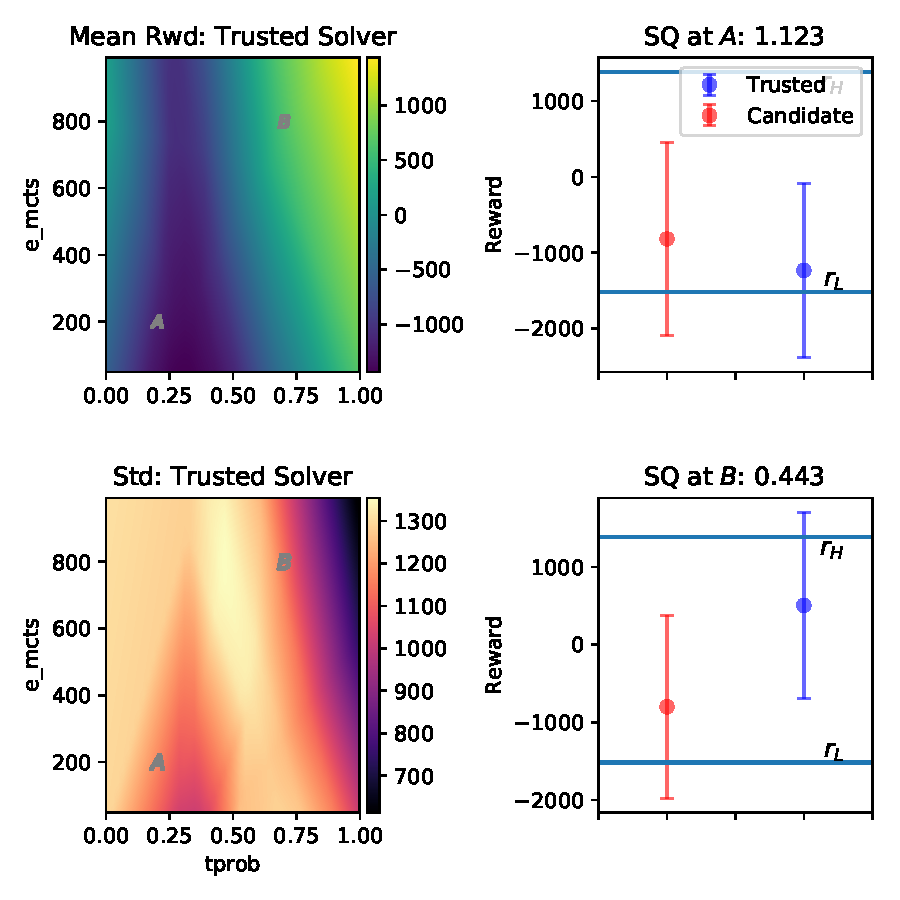
\includegraphics[width=0.9\linewidth]{Figures/transition_e_vary_e_mctstprob_bad.pdf}
    \caption{Using a solver with depth 1}
    \label{fig:tprob}
\end{figure}
